% Created by tikzDevice version 0.12
% !TEX encoding = UTF-8 Unicode
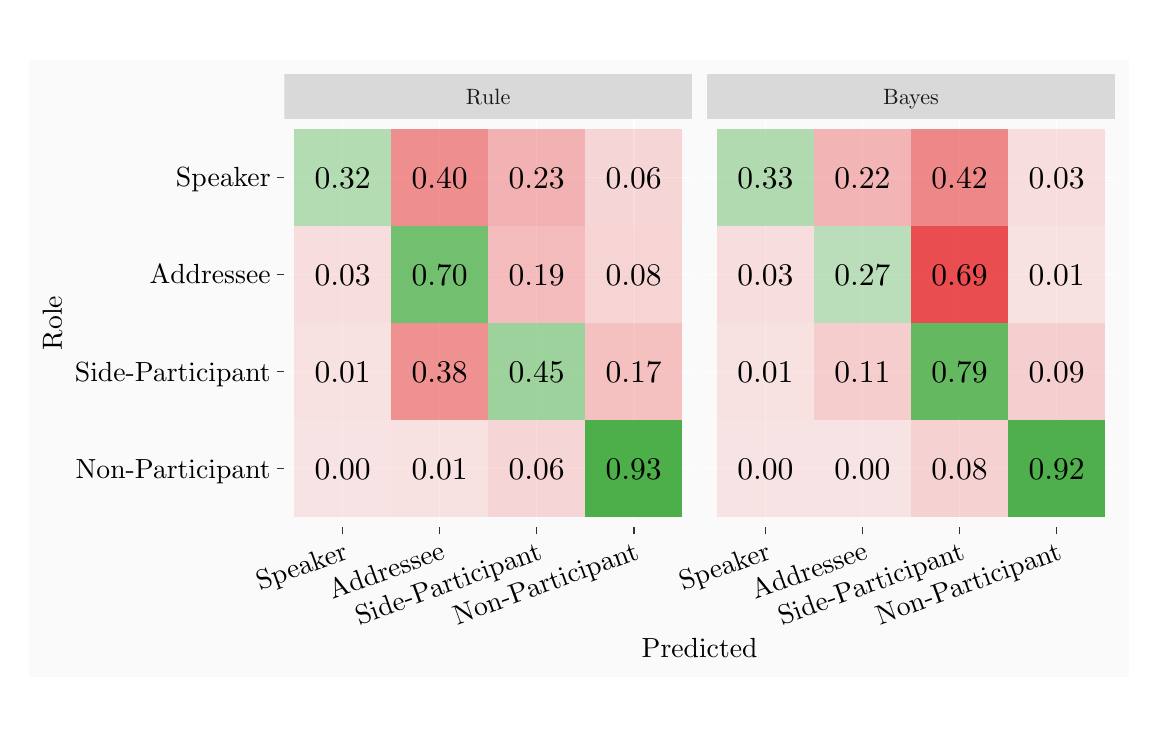
\begin{tikzpicture}[x=1pt,y=1pt]
\definecolor{fillColor}{RGB}{255,255,255}
\path[use as bounding box,fill=fillColor,fill opacity=0.00] (0,0) rectangle (398.34,246.17);
\begin{scope}
\path[clip] (  0.00, 11.30) rectangle (398.34,234.87);
\definecolor{drawColor}{RGB}{255,255,255}
\definecolor{fillColor}{gray}{0.98}

\path[draw=drawColor,line width= 0.6pt,line join=round,line cap=round,fill=fillColor] (  0.00, 11.30) rectangle (398.34,234.87);
\end{scope}
\begin{scope}
\path[clip] ( 92.74, 65.82) rectangle (240.04,213.12);
\definecolor{drawColor}{RGB}{255,255,255}

\path[draw=drawColor,line width= 0.6pt,line join=round] ( 92.74, 86.86) --
	(240.04, 86.86);

\path[draw=drawColor,line width= 0.6pt,line join=round] ( 92.74,121.93) --
	(240.04,121.93);

\path[draw=drawColor,line width= 0.6pt,line join=round] ( 92.74,157.00) --
	(240.04,157.00);

\path[draw=drawColor,line width= 0.6pt,line join=round] ( 92.74,192.07) --
	(240.04,192.07);

\path[draw=drawColor,line width= 0.6pt,line join=round] (113.78, 65.82) --
	(113.78,213.12);

\path[draw=drawColor,line width= 0.6pt,line join=round] (148.85, 65.82) --
	(148.85,213.12);

\path[draw=drawColor,line width= 0.6pt,line join=round] (183.92, 65.82) --
	(183.92,213.12);

\path[draw=drawColor,line width= 0.6pt,line join=round] (218.99, 65.82) --
	(218.99,213.12);
\definecolor{fillColor}{RGB}{77,175,74}

\path[fill=fillColor,fill opacity=0.40] ( 96.24,174.54) rectangle (131.32,209.61);
\definecolor{fillColor}{RGB}{228,26,28}

\path[fill=fillColor,fill opacity=0.48] (131.32,174.54) rectangle (166.39,209.61);
\definecolor{fillColor}{RGB}{228,26,28}

\path[fill=fillColor,fill opacity=0.32] (166.39,174.54) rectangle (201.46,209.61);
\definecolor{fillColor}{RGB}{228,26,28}

\path[fill=fillColor,fill opacity=0.16] (201.46,174.54) rectangle (236.53,209.61);
\definecolor{fillColor}{RGB}{228,26,28}

\path[fill=fillColor,fill opacity=0.13] ( 96.24,139.47) rectangle (131.32,174.54);
\definecolor{fillColor}{RGB}{77,175,74}

\path[fill=fillColor,fill opacity=0.78] (131.32,139.47) rectangle (166.39,174.54);
\definecolor{fillColor}{RGB}{228,26,28}

\path[fill=fillColor,fill opacity=0.28] (166.39,139.47) rectangle (201.46,174.54);
\definecolor{fillColor}{RGB}{228,26,28}

\path[fill=fillColor,fill opacity=0.17] (201.46,139.47) rectangle (236.53,174.54);
\definecolor{fillColor}{RGB}{228,26,28}

\path[fill=fillColor,fill opacity=0.11] ( 96.24,104.39) rectangle (131.32,139.47);
\definecolor{fillColor}{RGB}{228,26,28}

\path[fill=fillColor,fill opacity=0.47] (131.32,104.39) rectangle (166.39,139.47);
\definecolor{fillColor}{RGB}{77,175,74}

\path[fill=fillColor,fill opacity=0.53] (166.39,104.39) rectangle (201.46,139.47);
\definecolor{fillColor}{RGB}{228,26,28}

\path[fill=fillColor,fill opacity=0.26] (201.46,104.39) rectangle (236.53,139.47);
\definecolor{fillColor}{RGB}{228,26,28}

\path[fill=fillColor,fill opacity=0.10] ( 96.24, 69.32) rectangle (131.32,104.39);
\definecolor{fillColor}{RGB}{228,26,28}

\path[fill=fillColor,fill opacity=0.11] (131.32, 69.32) rectangle (166.39,104.39);
\definecolor{fillColor}{RGB}{228,26,28}

\path[fill=fillColor,fill opacity=0.16] (166.39, 69.32) rectangle (201.46,104.39);
\definecolor{fillColor}{RGB}{77,175,74}

\path[fill=fillColor] (201.46, 69.32) rectangle (236.53,104.39);
\definecolor{drawColor}{RGB}{0,0,0}

\node[text=drawColor,anchor=base,inner sep=0pt, outer sep=0pt, scale=  1.14] at (113.78,188.15) {0.32};

\node[text=drawColor,anchor=base,inner sep=0pt, outer sep=0pt, scale=  1.14] at (148.85,188.15) {0.40};

\node[text=drawColor,anchor=base,inner sep=0pt, outer sep=0pt, scale=  1.14] at (183.92,188.15) {0.23};

\node[text=drawColor,anchor=base,inner sep=0pt, outer sep=0pt, scale=  1.14] at (218.99,188.15) {0.06};

\node[text=drawColor,anchor=base,inner sep=0pt, outer sep=0pt, scale=  1.14] at (113.78,153.08) {0.03};

\node[text=drawColor,anchor=base,inner sep=0pt, outer sep=0pt, scale=  1.14] at (148.85,153.08) {0.70};

\node[text=drawColor,anchor=base,inner sep=0pt, outer sep=0pt, scale=  1.14] at (183.92,153.08) {0.19};

\node[text=drawColor,anchor=base,inner sep=0pt, outer sep=0pt, scale=  1.14] at (218.99,153.08) {0.08};

\node[text=drawColor,anchor=base,inner sep=0pt, outer sep=0pt, scale=  1.14] at (113.78,118.01) {0.01};

\node[text=drawColor,anchor=base,inner sep=0pt, outer sep=0pt, scale=  1.14] at (148.85,118.01) {0.38};

\node[text=drawColor,anchor=base,inner sep=0pt, outer sep=0pt, scale=  1.14] at (183.92,118.01) {0.45};

\node[text=drawColor,anchor=base,inner sep=0pt, outer sep=0pt, scale=  1.14] at (218.99,118.01) {0.17};

\node[text=drawColor,anchor=base,inner sep=0pt, outer sep=0pt, scale=  1.14] at (113.78, 82.94) {0.00};

\node[text=drawColor,anchor=base,inner sep=0pt, outer sep=0pt, scale=  1.14] at (148.85, 82.94) {0.01};

\node[text=drawColor,anchor=base,inner sep=0pt, outer sep=0pt, scale=  1.14] at (183.92, 82.94) {0.06};

\node[text=drawColor,anchor=base,inner sep=0pt, outer sep=0pt, scale=  1.14] at (218.99, 82.94) {0.93};
\end{scope}
\begin{scope}
\path[clip] (245.54, 65.82) rectangle (392.84,213.12);
\definecolor{drawColor}{RGB}{255,255,255}

\path[draw=drawColor,line width= 0.6pt,line join=round] (245.54, 86.86) --
	(392.84, 86.86);

\path[draw=drawColor,line width= 0.6pt,line join=round] (245.54,121.93) --
	(392.84,121.93);

\path[draw=drawColor,line width= 0.6pt,line join=round] (245.54,157.00) --
	(392.84,157.00);

\path[draw=drawColor,line width= 0.6pt,line join=round] (245.54,192.07) --
	(392.84,192.07);

\path[draw=drawColor,line width= 0.6pt,line join=round] (266.58, 65.82) --
	(266.58,213.12);

\path[draw=drawColor,line width= 0.6pt,line join=round] (301.65, 65.82) --
	(301.65,213.12);

\path[draw=drawColor,line width= 0.6pt,line join=round] (336.72, 65.82) --
	(336.72,213.12);

\path[draw=drawColor,line width= 0.6pt,line join=round] (371.80, 65.82) --
	(371.80,213.12);
\definecolor{fillColor}{RGB}{77,175,74}

\path[fill=fillColor,fill opacity=0.42] (249.04,174.54) rectangle (284.12,209.61);
\definecolor{fillColor}{RGB}{228,26,28}

\path[fill=fillColor,fill opacity=0.31] (284.12,174.54) rectangle (319.19,209.61);
\definecolor{fillColor}{RGB}{228,26,28}

\path[fill=fillColor,fill opacity=0.51] (319.19,174.54) rectangle (354.26,209.61);
\definecolor{fillColor}{RGB}{228,26,28}

\path[fill=fillColor,fill opacity=0.13] (354.26,174.54) rectangle (389.33,209.61);
\definecolor{fillColor}{RGB}{228,26,28}

\path[fill=fillColor,fill opacity=0.13] (249.04,139.47) rectangle (284.12,174.54);
\definecolor{fillColor}{RGB}{77,175,74}

\path[fill=fillColor,fill opacity=0.36] (284.12,139.47) rectangle (319.19,174.54);
\definecolor{fillColor}{RGB}{228,26,28}

\path[fill=fillColor,fill opacity=0.77] (319.19,139.47) rectangle (354.26,174.54);
\definecolor{fillColor}{RGB}{228,26,28}

\path[fill=fillColor,fill opacity=0.11] (354.26,139.47) rectangle (389.33,174.54);

\path[fill=fillColor,fill opacity=0.11] (249.04,104.39) rectangle (284.12,139.47);
\definecolor{fillColor}{RGB}{228,26,28}

\path[fill=fillColor,fill opacity=0.20] (284.12,104.39) rectangle (319.19,139.47);
\definecolor{fillColor}{RGB}{77,175,74}

\path[fill=fillColor,fill opacity=0.87] (319.19,104.39) rectangle (354.26,139.47);
\definecolor{fillColor}{RGB}{228,26,28}

\path[fill=fillColor,fill opacity=0.19] (354.26,104.39) rectangle (389.33,139.47);
\definecolor{fillColor}{RGB}{228,26,28}

\path[fill=fillColor,fill opacity=0.10] (249.04, 69.32) rectangle (284.12,104.39);

\path[fill=fillColor,fill opacity=0.10] (284.12, 69.32) rectangle (319.19,104.39);
\definecolor{fillColor}{RGB}{228,26,28}

\path[fill=fillColor,fill opacity=0.18] (319.19, 69.32) rectangle (354.26,104.39);
\definecolor{fillColor}{RGB}{77,175,74}

\path[fill=fillColor,fill opacity=0.99] (354.26, 69.32) rectangle (389.33,104.39);
\definecolor{drawColor}{RGB}{0,0,0}

\node[text=drawColor,anchor=base,inner sep=0pt, outer sep=0pt, scale=  1.14] at (266.58,188.15) {0.33};

\node[text=drawColor,anchor=base,inner sep=0pt, outer sep=0pt, scale=  1.14] at (301.65,188.15) {0.22};

\node[text=drawColor,anchor=base,inner sep=0pt, outer sep=0pt, scale=  1.14] at (336.72,188.15) {0.42};

\node[text=drawColor,anchor=base,inner sep=0pt, outer sep=0pt, scale=  1.14] at (371.80,188.15) {0.03};

\node[text=drawColor,anchor=base,inner sep=0pt, outer sep=0pt, scale=  1.14] at (266.58,153.08) {0.03};

\node[text=drawColor,anchor=base,inner sep=0pt, outer sep=0pt, scale=  1.14] at (301.65,153.08) {0.27};

\node[text=drawColor,anchor=base,inner sep=0pt, outer sep=0pt, scale=  1.14] at (336.72,153.08) {0.69};

\node[text=drawColor,anchor=base,inner sep=0pt, outer sep=0pt, scale=  1.14] at (371.80,153.08) {0.01};

\node[text=drawColor,anchor=base,inner sep=0pt, outer sep=0pt, scale=  1.14] at (266.58,118.01) {0.01};

\node[text=drawColor,anchor=base,inner sep=0pt, outer sep=0pt, scale=  1.14] at (301.65,118.01) {0.11};

\node[text=drawColor,anchor=base,inner sep=0pt, outer sep=0pt, scale=  1.14] at (336.72,118.01) {0.79};

\node[text=drawColor,anchor=base,inner sep=0pt, outer sep=0pt, scale=  1.14] at (371.80,118.01) {0.09};

\node[text=drawColor,anchor=base,inner sep=0pt, outer sep=0pt, scale=  1.14] at (266.58, 82.94) {0.00};

\node[text=drawColor,anchor=base,inner sep=0pt, outer sep=0pt, scale=  1.14] at (301.65, 82.94) {0.00};

\node[text=drawColor,anchor=base,inner sep=0pt, outer sep=0pt, scale=  1.14] at (336.72, 82.94) {0.08};

\node[text=drawColor,anchor=base,inner sep=0pt, outer sep=0pt, scale=  1.14] at (371.80, 82.94) {0.92};
\end{scope}
\begin{scope}
\path[clip] ( 92.74,213.12) rectangle (240.04,229.37);
\definecolor{fillColor}{gray}{0.85}

\path[fill=fillColor] ( 92.74,213.12) rectangle (240.04,229.37);
\definecolor{drawColor}{gray}{0.10}

\node[text=drawColor,anchor=base,inner sep=0pt, outer sep=0pt, scale=  0.80] at (166.39,218.49) {Rule};
\end{scope}
\begin{scope}
\path[clip] (245.54,213.12) rectangle (392.84,229.37);
\definecolor{fillColor}{gray}{0.85}

\path[fill=fillColor] (245.54,213.12) rectangle (392.84,229.37);
\definecolor{drawColor}{gray}{0.10}

\node[text=drawColor,anchor=base,inner sep=0pt, outer sep=0pt, scale=  0.80] at (319.19,218.49) {Bayes};
\end{scope}
\begin{scope}
\path[clip] (  0.00,  0.00) rectangle (398.34,246.17);
\definecolor{drawColor}{gray}{0.20}

\path[draw=drawColor,line width= 0.6pt,line join=round] (113.78, 63.07) --
	(113.78, 65.82);

\path[draw=drawColor,line width= 0.6pt,line join=round] (148.85, 63.07) --
	(148.85, 65.82);

\path[draw=drawColor,line width= 0.6pt,line join=round] (183.92, 63.07) --
	(183.92, 65.82);

\path[draw=drawColor,line width= 0.6pt,line join=round] (218.99, 63.07) --
	(218.99, 65.82);
\end{scope}
\begin{scope}
\path[clip] (  0.00,  0.00) rectangle (398.34,246.17);
\definecolor{drawColor}{RGB}{0,0,0}

\node[text=drawColor,rotate= 20.00,anchor=base east,inner sep=0pt, outer sep=0pt, scale=  1.00] at (116.13, 54.39) {Speaker};

\node[text=drawColor,rotate= 20.00,anchor=base east,inner sep=0pt, outer sep=0pt, scale=  1.00] at (151.21, 54.39) {Addressee};

\node[text=drawColor,rotate= 20.00,anchor=base east,inner sep=0pt, outer sep=0pt, scale=  1.00] at (186.28, 54.39) {Side-Participant};

\node[text=drawColor,rotate= 20.00,anchor=base east,inner sep=0pt, outer sep=0pt, scale=  1.00] at (221.35, 54.39) {Non-Participant};
\end{scope}
\begin{scope}
\path[clip] (  0.00,  0.00) rectangle (398.34,246.17);
\definecolor{drawColor}{gray}{0.20}

\path[draw=drawColor,line width= 0.6pt,line join=round] (266.58, 63.07) --
	(266.58, 65.82);

\path[draw=drawColor,line width= 0.6pt,line join=round] (301.65, 63.07) --
	(301.65, 65.82);

\path[draw=drawColor,line width= 0.6pt,line join=round] (336.72, 63.07) --
	(336.72, 65.82);

\path[draw=drawColor,line width= 0.6pt,line join=round] (371.80, 63.07) --
	(371.80, 65.82);
\end{scope}
\begin{scope}
\path[clip] (  0.00,  0.00) rectangle (398.34,246.17);
\definecolor{drawColor}{RGB}{0,0,0}

\node[text=drawColor,rotate= 20.00,anchor=base east,inner sep=0pt, outer sep=0pt, scale=  1.00] at (268.94, 54.39) {Speaker};

\node[text=drawColor,rotate= 20.00,anchor=base east,inner sep=0pt, outer sep=0pt, scale=  1.00] at (304.01, 54.39) {Addressee};

\node[text=drawColor,rotate= 20.00,anchor=base east,inner sep=0pt, outer sep=0pt, scale=  1.00] at (339.08, 54.39) {Side-Participant};

\node[text=drawColor,rotate= 20.00,anchor=base east,inner sep=0pt, outer sep=0pt, scale=  1.00] at (374.15, 54.39) {Non-Participant};
\end{scope}
\begin{scope}
\path[clip] (  0.00,  0.00) rectangle (398.34,246.17);
\definecolor{drawColor}{RGB}{0,0,0}

\node[text=drawColor,anchor=base east,inner sep=0pt, outer sep=0pt, scale=  1.00] at ( 87.79, 83.41) {Non-Participant};

\node[text=drawColor,anchor=base east,inner sep=0pt, outer sep=0pt, scale=  1.00] at ( 87.79,118.49) {Side-Participant};

\node[text=drawColor,anchor=base east,inner sep=0pt, outer sep=0pt, scale=  1.00] at ( 87.79,153.56) {Addressee};

\node[text=drawColor,anchor=base east,inner sep=0pt, outer sep=0pt, scale=  1.00] at ( 87.79,188.63) {Speaker};
\end{scope}
\begin{scope}
\path[clip] (  0.00,  0.00) rectangle (398.34,246.17);
\definecolor{drawColor}{gray}{0.20}

\path[draw=drawColor,line width= 0.6pt,line join=round] ( 89.99, 86.86) --
	( 92.74, 86.86);

\path[draw=drawColor,line width= 0.6pt,line join=round] ( 89.99,121.93) --
	( 92.74,121.93);

\path[draw=drawColor,line width= 0.6pt,line join=round] ( 89.99,157.00) --
	( 92.74,157.00);

\path[draw=drawColor,line width= 0.6pt,line join=round] ( 89.99,192.07) --
	( 92.74,192.07);
\end{scope}
\begin{scope}
\path[clip] (  0.00,  0.00) rectangle (398.34,246.17);
\definecolor{drawColor}{RGB}{0,0,0}

\node[text=drawColor,anchor=base,inner sep=0pt, outer sep=0pt, scale=  1.00] at (242.79, 18.75) {Predicted};
\end{scope}
\begin{scope}
\path[clip] (  0.00,  0.00) rectangle (398.34,246.17);
\definecolor{drawColor}{RGB}{0,0,0}

\node[text=drawColor,rotate= 90.00,anchor=base,inner sep=0pt, outer sep=0pt, scale=  1.00] at ( 12.39,139.47) {Role};
\end{scope}
\end{tikzpicture}
